\documentclass{article}
\usepackage[utf8]{inputenc}
\usepackage{amsmath, amsfonts, amsthm, amssymb}  % Some math symbols
\usepackage{natbib}
\usepackage{color}
\usepackage{graphicx}
\usepackage{multicol}
\usepackage[hidelinks]{hyperref}
\graphicspath{{images/}}
\title{The IBIC Shiny QA app}
\date{April 25, 2017}
\begin{document}
	
\begin{center}
	\LARGE{The IBIC Shiny QA app}
\end{center}
\section{Overview}
For the Udall project, brain scan quality assurance procedures will be primarily completed using an R Shiny application, as a convenient and visually appealing alternative to command-line-based methods. Through this guide, we will cover how the app works, how to distinguish between ``good" and ``bad'' images, and how to add warning checks. \\\\
Here's what the app looks like when it's first opened, and how it works: \newline
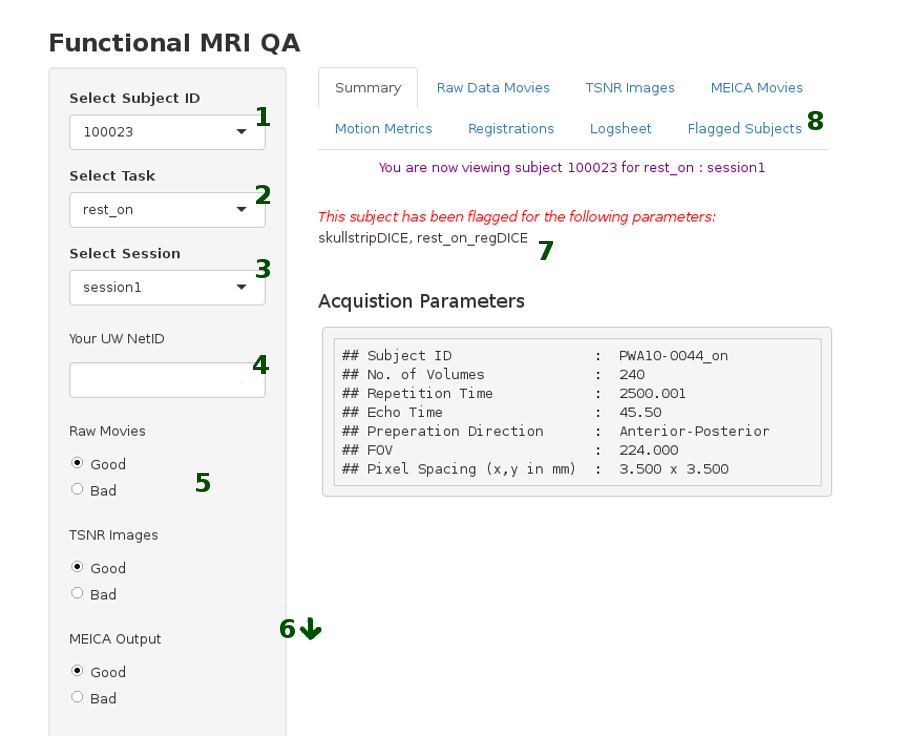
\includegraphics[scale=0.4]{shiny_summary_numbered.png}

\begin{enumerate}
	\item \textbf{Subject ID}: All the scanned subjects are listed here. Choose different items on the drop-down menu to switch between subjects.
	\item \textbf{Tasks}: Every PD subject will have four different tasks to be checked. Control subjects will have only the ``on'' tasks. 
	\item \textbf{Session}: Currently, all subjects have only session1; as the study progresses, more sessions will be added. 
	\item \textbf{UW NetID}: Input your NetID here to submit a QA report.
	\item \textbf{Good/Fair/Bad}: For each measure, find the corresponding tab and select ``good'', ``bad'', or ``fair'' based on quality of the data. 
	\item \textbf{Submit a log}: Scroll down to the bottom of the sidebar, and click ``submit''. If you accidentally submit an incorrect log, go to ShinyQA/output/ and remove your most recent entry. 
	\item \textbf{Warnings}: If warnings show up, pay especially close attention to the scans they mention. These images are more likely to be problematic.
	\item \textbf{Flagged Subjects}: These are the subjects that have warnings. 
\end{enumerate}
Next we will take a look at how to distinguish between ``good'' and ``bad'' images. 
\section{Checking Brain Scan Quality}
Here are some examples of bad and good images. The bad images are unusable as they are. However, in some cases procedures can be taken to rectify certain issues. \\\\
\textbf{fMRI Movies:}
\\\\
\noindent\begin{minipage}{0.45\textwidth}
	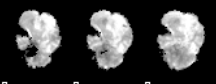
\includegraphics[scale=0.79]{bad_image2.png}
\end{minipage}%
\hfill%
\begin{minipage}{0.45\textwidth}
	Significant chunks of the brain are omitted, because the scanner has failed to pick up all of the brain.\\
	\textbf{The fix:} none
\end{minipage}\newline\newline
\noindent\begin{minipage}{0.45\textwidth}
	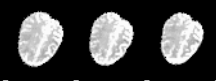
\includegraphics[scale=0.79]{bad_image3.png}
\end{minipage}%
\hfill%
\begin{minipage}{0.45\textwidth}
	The brain is significantly tilted. \\
	\textbf{The fix:} PROC
\end{minipage}
\noindent\begin{minipage}{0.45\textwidth}
	
\includegraphics[scale=1.115]{bad_image5.png}
\end{minipage}%
\hfill%
\begin{minipage}{0.45\textwidth}
	A movie has unexpected \\scrolling movements. \\
	\textbf{The fix:} Scrap two volumes from the beginning and end of the movie, then merge frames for full images.
\end{minipage}\\\\\\
\noindent\begin{minipage}{0.45\textwidth}
	This is a usable image. No artifacts are present, and the whole brain is represented.
\end{minipage}%
\hfill%
\begin{minipage}{0.45\textwidth}
	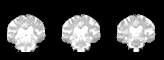
\includegraphics[scale=1.045]{meica_good2.png}
\end{minipage}\\\\\\\\
\textbf{TSNR:}\\
Bad TSNR images may appear blurred. Contrast may be incorrectly adjusted so that distinct brain structures are indistinguishable. \\\\
\noindent\begin{minipage}{0.45\textwidth}
	Brain structures are clear, and there is no obvious blurring. This is a good image.
\end{minipage}%
\hfill%
\begin{minipage}{0.45\textwidth}
	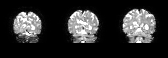
\includegraphics[scale=1.025]{tsnr_good2.png}
\end{minipage}\\\\
\noindent\begin{minipage}{0.45\textwidth}
	This is a good image. Contrast here is good, with clarity in regards to brain structures. 
\end{minipage}%
\hfill%
\begin{minipage}{0.45\textwidth}
	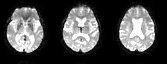
\includegraphics[scale=1.025]{tsnr_good1.png}
\end{minipage}\\\\\\
\textbf{Registration:}\\\\
\noindent\begin{minipage}{0.45\textwidth}
	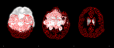
\includegraphics[scale=1.5]{badreg3.png}
\end{minipage}%
\hfill%
\begin{minipage}{0.45\textwidth}
	Registration appears to barely try matching the actual brain. \\
	\textbf{The fix:} Re-run the registration processing. If the tracing is still terribly off, PROC
\end{minipage}\\\\
\noindent\begin{minipage}{0.45\textwidth}
	Registration looks \emph{about} right. This image is acceptable. 
\end{minipage}%
\hfill%
\begin{minipage}{0.45\textwidth}
	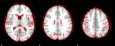
\includegraphics[scale=1.485]{reg_good1.png}
\end{minipage}
\noindent\begin{minipage}{0.45\textwidth}
	Registration follows the brain's contours fairly accurately. This image is good. 
\end{minipage}%
\hfill%
\begin{minipage}{0.45\textwidth}
	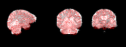
\includegraphics[scale=1.355]{reg_good2.png}
\end{minipage}
\newpage
\noindent\textbf{Other issues to look out for:}\\\\
\noindent\begin{minipage}{0.3\textwidth}
	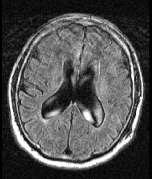
\includegraphics[scale=0.75]{T1_bad1.png}
\end{minipage}%
\hfill%
\begin{minipage}{0.6\textwidth}
	T1 images: Some ringing and blurriness can be perceived in the brain. This is due to motion during the T1 scan. No fix is currently available. 
\end{minipage}\\\\
\noindent\begin{minipage}{0.3\textwidth}
	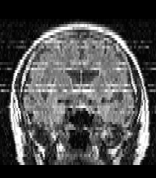
\includegraphics[scale=0.735]{T1_bad2.png}
\end{minipage}%
\hfill%
\begin{minipage}{0.6\textwidth}
	T1 images: Noise from the scanner itself appear on the image. Nothing can be done about these static-y artifacts, so this image is unusable. 
\end{minipage}
\\\\
For even more examples of what can go wrong with brain images, see \href{http://cbs.fas.harvard.edu/usr/mcmains/CBS_MRI_Quality_Control_Workshop.pdf}{\color{cyan}{this}}.
\section{Warnings}
\textbf{Skullstrip DICE:} \\
e.g. skullstripDICE, rest\_on\_regDICE\\
These warnings indicate that the process of stripping the skull away from T1 images might not have been entirely successful. Pay especially close attention to skullstripped images during QA.\\\\
\textbf{Scan parameters:} \\
e.g. RS\_off\_slices, ME\_Task\_on\\
These warnings indicate that the scan parameters for this subject's scan were incorrectly set.\\\\
\textbf{Motion Metrics:} \\
e.g. axcpt\_on\_dvarsvals\_e002\_mean, abs\_mean\_displacement, percent\_outliers\\
 Warnings generated for motion metrics are primarily an indication that something may be wrong with task-relevant brain images due to too much motion; in movies, look for excessive motion. In still images, look for blurriness. 

\section{Updating/Adding Warnings to the App}
Each subject's warnings appear near the top of their summary page. Additionally, warnings for all subjects can be observed in the flagged subjects tab. These warnings are read from the file \texttt{QA/\textbf{SUBJECTID}\_QA\_stats.csv} in each subject's directory where \texttt{SUBJECTID} is variable. The file is structured as follows:
\begin{align*}
	& \texttt{measure,data,flag}\\
	& \texttt{RS\_off\_slices,37,0}\\
	& \texttt{RS\_off\_echoes,3,0}\\
	& \texttt{RS\_off\_dyn\_scans,240,0}\\
	& \texttt{RS\_off\_FOV\_RL,224.000,0}\\
	& ...
\end{align*}
and so on. When a flag = 1, the corresponding measure's name is displayed in the app as a warning. The data column contains the measure's quantitative value. \\\\
To generate these .csv files, run \texttt{make QA/\textbf{SUBJECTID}\_QA\_stats.csv} in each subject's directory. Alternatively, one can also call the \texttt{generate\_QA\_stats} script directly with two arguments \texttt{SUBJECTID} and \texttt{SESSIONNO} where the latter is the desired session number. Here is the default location of the QA csv-generating script:
\begin{center}
	\texttt{/mnt/panuc/IBIC\_Pipelines/ShinyQA/generate\_QA\_stats}
\end{center}
\textbf{Altering flag thresholds:} All thresholds should be numerical values that are global fields that can be found in the beginning of the script. To change the thresholds, simply edit these existing fields and regenerate all subjects' csv files after the update. \\\\
\textbf{Adding potential warnings:} Follow the output format (measure,data,flag) as shown above when adding to the script \texttt{generate\_QA\_stats}. This script generates flags in two stages, for task-independent and then task-dependent measures. Measures are task-dependent if they can be categorized as either \texttt{rest\_on}, \texttt{rest\_off}, \texttt{axcpt\_on}, or \texttt{axcpt\_off}. Add flag computations under the appropriate stage. Then re-generate the csvs for all subjects under the new script. \\\\
\textbf{Future Improvements:} Whenever a QA stats csv file is updated, it is regenerated from scratch. As the flags being generated are currently inexpensive to compute, regeneration is quick. However, if more time-consuming flags are to be computed in the future, it would be a good idea to look into caching such flags in such a way that they need not be recomputed. 

\end{document}
